\documentclass{article}

\usepackage[top=1in, bottom=1.5in, left=1.2in, right=1.2in]{geometry}
\usepackage{graphicx}
\usepackage{afterpage}
\usepackage{amsmath}


\title{\textbf{
    APS 5 - Análise da frequência de ocorrências de terremotos próximos à Nicarágua
}}
\author{Grupo 8 - Gustavo Barroso Souza Cruz, Ian Cordibello Desponds}
\date{\today}


\begin{document}
    \maketitle
    \section*{Contexto}
    
    Os terremotos ou abalos sísmicos são fenômenos naturais que ocorrem quando há um deslocamento e choque de placas tectônicas.
    A grande maioria desses eventos ocorre nas zonas de contato entre placas, que são chamadas de falhas geológicas.
    É interessante notar que os abalos sísmicos são eventos independentes entre si, ou seja, a ocorrência de um terremoto 
    não influencia na ocorrência de outro.

    A Nicarágua, está localizada no centro da América Central, onde ocorre a convergência de quatro placas tectônicas: a placa do Caribe,
    a placa de Cocos, a placa de Nazca e a placa Norte-Americana (como pode ser observado na foto abaixo). Por conta disso, a região em 
    volta deste país tem uma grande atividade sísmica, registrando terremotos frequentemente.
    \\

    \begin{figure}[h]
        \centering
        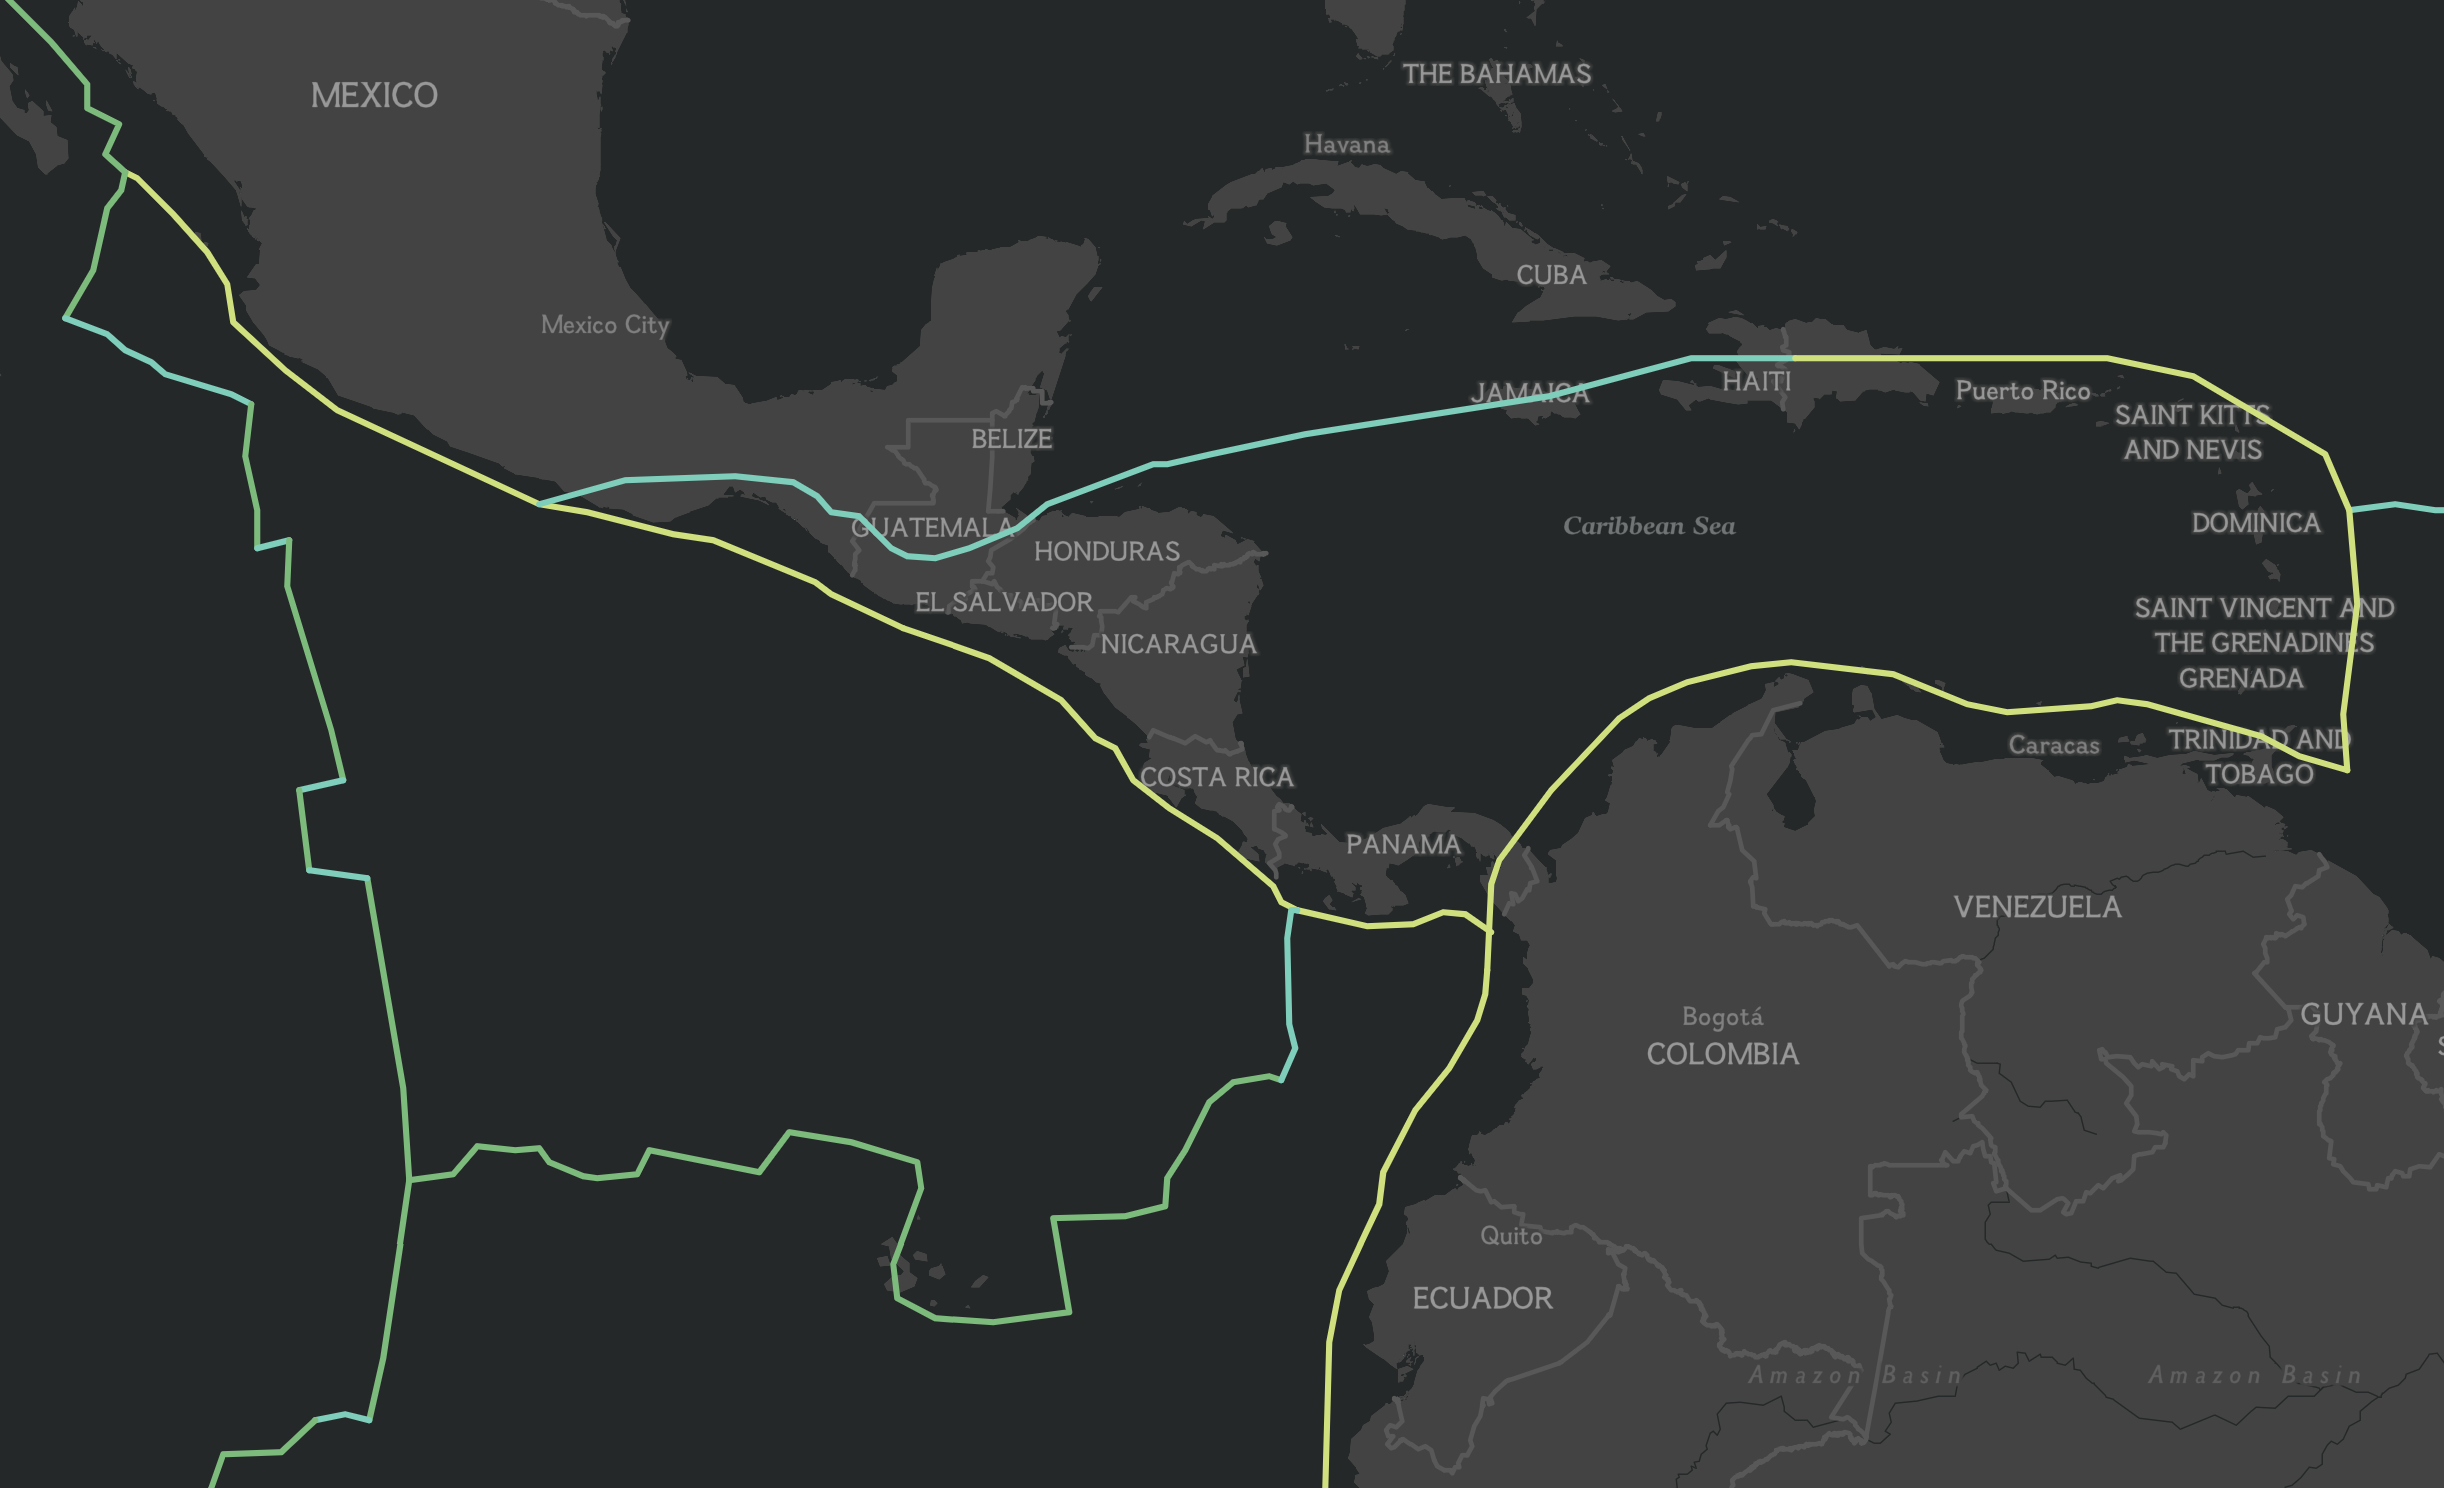
\includegraphics[width=0.69\textwidth]{nicaragua.png}
        \caption{Localização da Nicarágua e limites das placas tectônicas}
        \label{fig:my_label}
    \end{figure}

    \section*{A análise}

    \subsection*{Tratando os Dados}

    A base de dados só contém terremotos de magnitude maior ou igual a 5.5 na escala Richter, que são considerados terremotos moderados.
    Para definir a área que estamos analisando, definimos as coordenadas da capital da Nicarágua, Manágua, como o centro e determinamos que
    a área de interesse é um quadrado de lado 10 graus de latitude e longitude. Filtramos o dataframe para que contenha apenas eventos
    ocorridos dentro dessa área e fizemos a análise a partir desse novo dataframe filtrado.\\

    \subsection*{Estimando o Parâmetro}

    O parâmetro que estamos interessados é o tempo médio entre a ocorrência de eventos ($\mu$). Para encontrá-lo, primeiro
    calculamos o nosso $\lambda$, que é a média de ocorrências de terremotos por mês (assumindo um mês de 30 dias). Encontramos
    que o $\lambda$ é de aproximadamente 0.571 eventos por mês.

    Como se trata de intervalo de tempo entre eventos, o modelo mais adequado é o modelo da distribuição exponencial. Assim
    ficou a distribuição de probabilidade do nosso modelo:\\

    \begin{figure}[h]
        \centering
        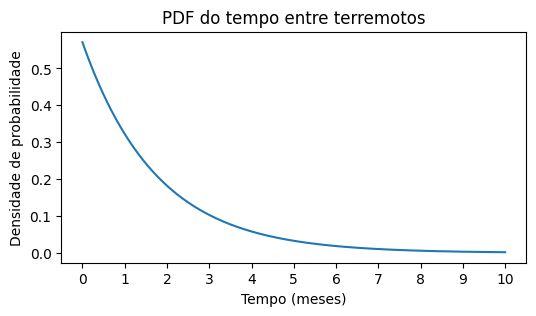
\includegraphics[width=0.5\textwidth]{pdf_expon_terremotos.png}
        \caption{Função de densidade de probabilidade da distribuição exponencial}
    \end{figure}


    Por se tratar de uma distribuição exponencial, o parâmetro $\mu$ é o inverso do $\lambda$. Ou seja, $\mu$ pode ser calculado 
    como $\frac{1}{\lambda}$. S o valor de $\lambda$ encontrado, obtemos que o $\mu$ 
    é de aproximadamente 1.75 meses.\\


    \subsection*{Limites do intervalo de confiança}
    
    Para um intervalo de confiança de 95\% ($\alpha = 0.05$), queremos encontrar os limites inferior e superior do intervalo.
    Usando a função \textit{st.expon.ppf} do \textit{scipy}, encontramos que o limite inferior é de aproximadamente 0.44 meses
    entre eventos e o limite superior é de aproximadamente 6.45 meses entre eventos. Assim ficou o intervalo de confiança:

    \begin{figure}[h]
        \centering
        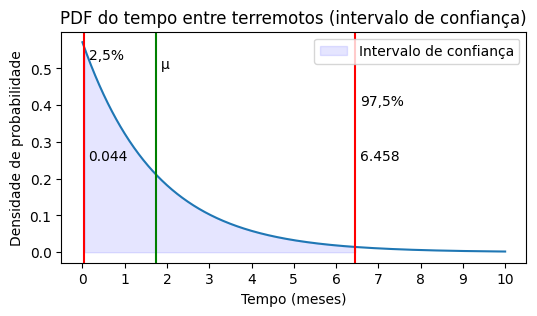
\includegraphics[width=0.5\textwidth]{pdf_expon_terremotos_IC.png}
        \caption{Intervalo de confiança de 95\%}
    \end{figure}

    Ao observar o intervalo de confiança, interpretamos que, com um nível de confiança de 95\%, o intervalo de tempo entre terremotos
    na região de interesse deve estar entre 0.44 e 6.45 meses.\\


    \section*{Autoavaliação - Conceito A}

    Nós acreditamos que merecemos o conceito A pois, seguindo a rubrica do trabalho, encontramso o parâmetro $\mu$ da distribuição,
    identificamos que a distribuição ideal era a exponencial e usamos o Teorema do Limite Central para encontrar o intervalo de confiança
    para o parâmetro encontrado o interpretamos. Ademais, fomos além do que foi pedido e demos um breve contexto do fenômeno observado e desenhamos
    gráficos para melhor visualização dos resultados. \\


    \section*{Referências}

    [1] Significant Earthquakes, 1965-2016 : https://www.kaggle.com/datasets/usgs/earthquake-database
    \

    \noindent[2] Tectonic Plate Boundaries (NatGeo) : https://mapmaker.nationalgeographic.org/map/692b3ff1cd60449da2e882085f631c4e



\end{document}
